Il \textbf{grid computing} è un'architettura di calcolo distribuito che
collega computer sparsi geograficamente allo scopo di condividere risorse e
potenza di calcolo per raggiungere uno scopo condiviso.
Attualmente, il più grande sistema grid al mondo è Worldwide LHC Computing
Grid (WLCG). Questa è una collaborazione internazionale che coinvolge oltre
170 centri di calcolo sparsi in più di 40 nazioni. Lo scopo del WLCG è fornire
l'infrastruttura computazionale necessaria per gestire i dati generati dagli
esperimenti effettuati con il Large Hadron Collider (LHC) \cite{WLCG2023}.

Come mostrato nella figura \ref{fig:WLCG_tier_hierarchy}, i centri di calcolo
all'interno del WLCG sono strutturati secondo il modello MONARC, che li
organizza in un sistema gerarchico di livelli, noti come Tier, ciascuno dei
quali ha funzioni e responsabilità ben definite.
In questo contesto si colloca il centro nazionale delle tecnologie
informatiche e telematiche (CNAF), che ospita il Tier-1 per tutti e quattro
gli esperimenti del LHC. Oltre agli esperimenti LHC, vengono supportati presso
il CNAF gli esperimenti non-LHC di astrofisica delle particelle e fisica dei
neutrini \cite{Bortolotti2012}.

\begin{figure}[ht]
    \centering
    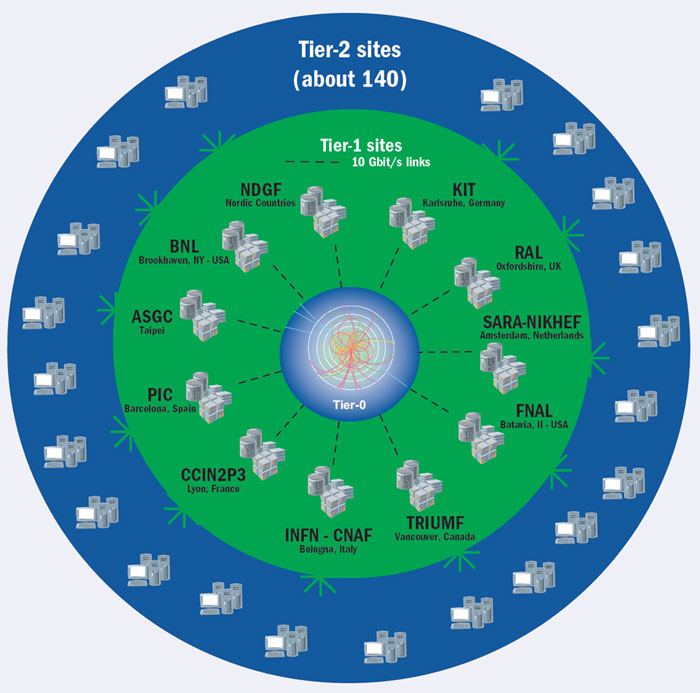
\includegraphics[width=0.75\linewidth]{WLCG_tier_hierarchy}
    \caption{Struttura gerarchica del WLCG \protect\cite{dalpra2019}}
    \label{fig:WLCG_tier_hierarchy}
\end{figure}

Il CNAF offre più di 46000 core distribuiti su 960 host fisici per un totale di
circa $630$ kHS06\footnote{metrica per misurare le prestazioni della CPU,
sviluppata dal gruppo di lavoro HEPiX. È utilizzata per confrontare le risorse
di calcolo in ambito scientifico.} di potenza di calcolo \cite{hepix2022}.
L'allocazione di queste risorse segue il paradigma del \textbf{High-Throughput
Computing} (HTC), dove a differenza dell'High-Performance Computing, che mira
a eseguire calcoli ad alta velocità, l'obiettivo dell'HTC è massimizzare il
numero di operazioni compiute su un periodo di tempo prolungato. 

Ogni esperimento ha almeno una coda dedicata e le risorse di calcolo sono
gestite centralmente da un unico batch system (HTCondor) \cite{cnaf_calcolo}.
In questo contesto, un \textbf{job} rappresenta un'unità di lavoro che un
utente vuole eseguire. Questa può essere una qualsiasi operazione che richieda
risorse computazionali. Una volta sottomesso, il job viene accodato da un
batch system e attende la sua schedulazione in base ad algoritmi di fairshare.
Questi algoritmi assicurano che le risorse computazionali siano distribuite
equamente tra tutti gli utenti e le varie code, impedendo che un singolo
utente o coda possa monopolizzare tutte le risorse o che una coda soffra di
\textit{starvation}\footnote{Si riferisce a una situazione in cui un job non
viene mai eseguito perché sono presenti job con priorità più alta.}.


In media, ogni giorno vengono eseguiti 100000 jobs batch, e le risorse di
calcolo sono utilizzate 24×7 dai vari esperimenti scientifici.


Una serie di dati è una sequenza ordinata di punti dati, ed esprime la
dinamica di un certo fenomeno nel tempo. Quando questi dati sono ordinati 
in base al tempo, si parla di una \textbf{serie temporale}. Indipendentemente dal
criterio utilizzato per ordinarli, i punti dati sono registrati seguendo
intervalli di tempo equispaziati. Le serie temporali
possono essere di due tipi: \textbf{univariate}, che coinvolgono una singola variabile
misurata nel tempo, e \textbf{multivariate}, dove più variabili sono misurate
contemporaneamente.


\begin{figure}[ht]
    \centering
    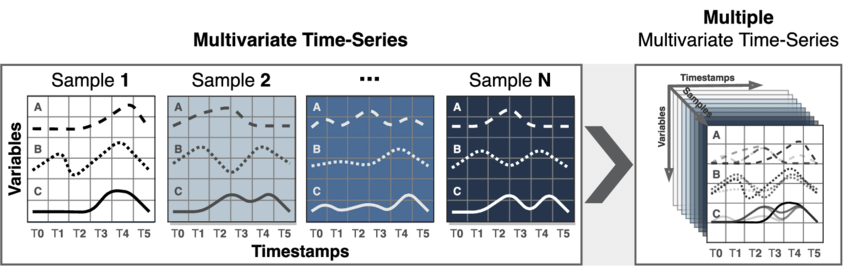
\includegraphics[width=0.75\linewidth]{A-multiple-multivariate-time-series}
%\includegraphics[width=5cm]{figura.eps}%inserisce una figura larga 5cm
% inserisce la legenda ed etichetta
% la figura con \label{fig:prima}
    \caption[legenda elenco figure]{mettere riferimento}\label{fig:prima}
\end{figure}
